\section{Genetic Algorithm}

A Genetic Algorithm (GA) is a search heuristic that is based on Darwin's theory of natural evolution. Darwin theorized that over a period of time a population of individuals would naturally mate and create offspring that were better than themselves. He suggests that not all individuals are created equally and that eventually the weaker individuals would die off. This same principle can be applied to a search algorithm. A GA contains a population of individuals that are evolved to find improved candidate solutions.

The individuals of a GA represent possible candidate solutions to the problem. Individuals are refered to as chromosomes. Typically a chromosome is represented as an array where each index of the array represents a property of the candidate solution. There are no restrictions to the encoding of a chromosome but each property of the chromosome must be independant from the others. The simplest example of a representation is a binary array of 1's and 0's, as shown in Figure~\ref{figure:sampleChromosome}.

\begin{figure}
  \label{figure:sampleChromosome}
  \centering
  \begin{tabular}{ | l | l | l | l | l | l | l | l | }
    \hline
    0 & 1 & 1 & 0 & 1 & 0 & 1 & 0 \\
    \hline
  \end{tabular}
  \caption{Simple Chromosome Represention}
\end{figure}

Finding a representation is only the first step in creating a genetic algorithm. The next step is to define your set of operators. A GA consists of multiple operators that assist in the evolution of the population. Figure~\ref{figure:gaFlowchart} depicts the flowchart of a genetic algorithm and where each genetic operation is performed.

\begin{figure}
	\centering
	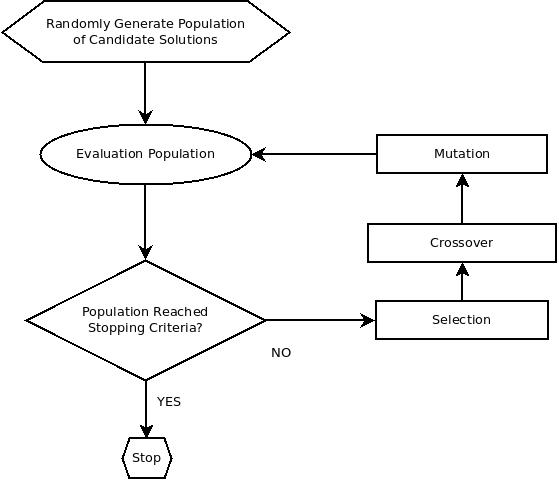
\includegraphics[bb=0 0 559 481,scale=0.5]{figures/GA.jpeg}
	\caption{Population Individual Modification}
	\label{figure:gaFlowchart}
\end{figure}

\subsection{Genetic Operators}

Each of the following operators represent a piece of a genetic algorithm. They facilitate the evolutionary process in an effort to find better candidate solutions. Each of these operators has a unique purpose in the search algorthm but there are many different types of ways these goals can be carried out. Only a few of the different methods will be described in this work.

\textit{Evaluation Function}: This operator determines the fitness of an individual. Each individual is evaluated and given a fitness score to represent how well the individual performed on the problem. This operation is problem specific and can be very difficult to determine how a problem should be evaluated.

\textit{Selection Operator}: This operator is very important to the \textit{Crossover} and \textit{Mutation} operators. The idea behind this operator is to put selectionary pressure on the population. With respect to Darwin's Theor

\textit{Crossover Operator}:

\textit{Mutation Operator}:

\textit{Elitism Operator}:

% The GA has shown success in past studies in finding low-energy protein conformations. For example in~\cite{comte2010bioinspired} a GA is used to search through a continuous space in order to find low-energy protein conformations. This bears a similarity to this problem, as it is a continuous search space produces 3D structures. Also a population based search is important so that a number of candidate solutions are available, as some structures may be chemically unreasonable.